\begin{tikzpicture}[remember picture, scale=\modDGHyperScale]
% dummy
\coordinate[overlay] (v-coord-0-0) at (3.7847, 4.4663) {};
\coordinate[overlay] (v-coord-1-0) at (6.527, 4.9191) {};
\coordinate[overlay] (v-coord-2-0) at (5.5445, 2.3333) {};
\coordinate[overlay] (v-coord-4-0) at (0.81514, 2.5651) {};
\coordinate[overlay] (v-coord-5-0) at (3.5574, 3.0178) {};
\coordinate[overlay] (v-coord-6-0) at (2.575, 0.43212) {};
\coordinate[overlay] (v-coord-3-0) at (5.2847, 3.9117) {};
\coordinate[overlay] (v-coord-7-0) at (2.3151, 2.0105) {};

% id = 0, graphName = g_{0}
\node[modStyleDGHyperVertex, at=(v-coord-0-0)] (v-0-0) {\includegraphics[scale=\modDGHyperImageScale] {\modInputPrefix/out/001_g_0_11311100.pdf}\\{$\mathrm{g_{0}}$}};
% id = 1, graphName = g_{1}
\node[modStyleDGHyperVertex, at=(v-coord-1-0)] (v-1-0) {\includegraphics[scale=\modDGHyperImageScale] {\modInputPrefix/out/002_g_1_11311100.pdf}\\{$\mathrm{g_{1}}$}};
% id = 2, graphName = g_{2}
\node[modStyleDGHyperVertex, at=(v-coord-2-0)] (v-2-0) {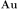
\includegraphics[scale=\modDGHyperImageScale] {\modInputPrefix/out/003_g_2_11311100.pdf}\\{$\mathrm{g_{2}}$}};
% id = 4, graphName = g_{3}
\node[modStyleDGHyperVertex, at=(v-coord-4-0)] (v-4-0) {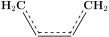
\includegraphics[scale=\modDGHyperImageScale] {\modInputPrefix/out/004_g_3_11311100.pdf}\\{$\mathrm{g_{3}}$}};
% id = 5, graphName = g_{4}
\node[modStyleDGHyperVertex, at=(v-coord-5-0)] (v-5-0) {\includegraphics[scale=\modDGHyperImageScale] {\modInputPrefix/out/005_g_4_11311100.pdf}\\{$\mathrm{g_{4}}$}};
% id = 6, graphName = g_{5}
\node[modStyleDGHyperVertex, at=(v-coord-6-0)] (v-6-0) {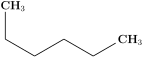
\includegraphics[scale=\modDGHyperImageScale] {\modInputPrefix/out/006_g_5_11311100.pdf}\\{$\mathrm{g_{5}}$}};
% id = 3{ 'g_{0}' 'g_{1}' }, { 'g_{2}' }
\node[modStyleDGHyperEdge, at=(v-coord-3-0)] (v-3-0) {};
% id = 7{ 'g_{3}' 'g_{4}' }, { 'g_{5}' }
\node[modStyleDGHyperEdge, at=(v-coord-7-0)] (v-7-0) {};
% id = 3{ 'g_{0}' 'g_{1}' }, { 'g_{2}' }
\path[modStyleDGHyperConnector] (v-0-0) to (v-3-0);
\path[modStyleDGHyperConnector] (v-1-0) to (v-3-0);
\path[modStyleDGHyperConnector] (v-3-0) to (v-2-0);
% id = 7{ 'g_{3}' 'g_{4}' }, { 'g_{5}' }
\path[modStyleDGHyperConnector] (v-4-0) to (v-7-0);
\path[modStyleDGHyperConnector] (v-5-0) to (v-7-0);
\path[modStyleDGHyperConnector] (v-7-0) to (v-6-0);
\end{tikzpicture}%
